Como exposto na subseção anterior~\ref{subsec:limites-da-camada-de-p-convolucao}, a camada \emph{PConv} possui alguns casos de desvantagens.
E, propõe-se duas novas camadas morfológicas baseadas nos princípios fundamentais da \emph{PConv} para fazê-las compatíveis com a morfologia matemática de tons de cinza geral.

\subsection{Apresentando à operação $\mathcal{L}$Morph}
\label{subsec:introduzindo-a-operacao-lmorph}

Com objetivo de contornar as funções não diferenciáveis $\min$ e $\max$ substituindo por aproximações diferenciáveis e suáveis, propõe-se a definição de $\mathcal{L}$Morph, inspirada na morfologia baseada na média de Lehmer.
Explorando o comportamento morfológico apresentado da camada $PConv$, apresenta-se:

% Equation 11
\begin{equation}
    \mathcal{L}\text{Morph}(f, w, p)(x) =
    \frac{\sum_{y \in W(x)} \big{(}f(y)w(x-y)\big{)}^{p+1}}{\sum_{y \in W(x)} \big{(}f(y)w(x-y)\big{)}^{p}}
    \label{eq:equation11}
\end{equation}
\\
onde $w: W \to \mathbb{R}^{+}$ é a função estruturante e $p \in \mathbb{R}$.
Interpretando a equação~\ref{eq:equation11} em relação a equação~\ref{eq:equation5} como $f(y) = f(y)w(x-y)$ e $1$ substituindo os valores de $w$ para que, de forma assintótica, reproduza-se o comportamento

% Equation 12
\begin{equation}
    \lim_{p \to +\infty} \mathcal{L}\text{Morph}(f, w, p)(x) =
    \sup_{y \in E}\Big{\{} f(y) + b(x - y)\Big{\}} = (f \oplus w)(x)
    \label{eq:equation12}
\end{equation}

% Equation 13
\begin{equation}
    \lim_{p \to +\infty} \mathcal{L}\text{Morph}(f, w, p)(x) =
    \inf_{y \in E}\Big{\{} f(y) + b(x - y)\Big{\}} = (f \ominus -w)(x)
    \label{eq:equation13}
\end{equation}

Pela mudança de sinal de $p$ é pode atingir uma pseudo-dilatação ou pseudo-erosão quando, respectivamente, $p > 0$ e $p < 0$.
Na prática, tal efeito é alcançado quando $|p| > 20$.

\begin{figure}[h]
    \caption{Linha superior: imagem de entrada, elemento estruturante não plano, dilatação alvo, erosão alvo. Linha média: pseudo-dilatação de $\mathcal{L}$Morph por incremento do valor de $p$. Linha inferior: pseudo-erosão de $\mathcal{L}$Morph por decremento do valor de $p$.}
    \centering
    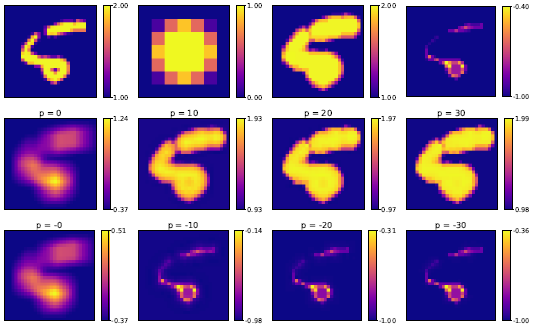
\includegraphics[scale=0.9]{images/LMorph}
    \label{fig:lmporh}
\end{figure}

Ressalta-se que as limitações de CHM são compartilhadas com $\mathcal{L}$Morph e que, por isso, a pseudo-erosão demonstrada na equação~\ref{eq:equation13} possui o elemento estruturante $w$ negativo.
Decorre-se que $\big{(}f(y)w(x-y)\big{)}$ tem as limitações de $f(x)$ citadas na seção~\ref{subsec:limites-da-camada-de-p-convolucao}, além da necessidade de reescalonamento.

\subsection{Introdução a operação $\mathcal{S}$Morph}
\label{subsec:introducao-a-operacao-smorph}

A função \emph{softmax} leva como entrada um vetor $x$ de $n$ números reais e os normaliza dentro de uma distribuição de probabilidade proporcional aos exponenciais dos números de entrada.
Alguns componentes do vetor $x$ podem ser negativos, ou maiores que $1$; e não totatlizar $1$.
Mas, após a aplicação da função, cada componente estará no intervalo $[0, 1]$ e resultarão $1$ quando somados.
A função \emph{softmax} $\mathcal{S}(x): \mathbb{R}^{n} \to [0, 1]^{n}$ é definida para $n > 1$ pela formula

% Equation 14
\begin{equation}
    \mathcal{S}(x_{i}) = \frac{e^{x_{i}}}{\sum_{j=1}^{n} e^{x_{j}}} \text{ para } i = 1, \dots, K
    \text{ e } x = (x_{i}, \dots, x_{n}) \in \mathbb{R}^{n}.
    \label{eq:equation14}
\end{equation}
\\
Ao invés de $e$, uma diferente base $b > 0$ pode ser usada.
Compete-se que se $0 > b > 1$, componentes de entrada menores resultarão em valores de sáida maiores.
Diminuir o valor de $b$ criará uma distribuição de probabilidade mais concentrada em torno das posições dos menores valores de entrada.
Por conseguinte, $b > 1$ resultará em valores de saídas maiores para os componentes de entrada maiores, e o aumento de $b$ implicará na concentração da distribuição de probabilidade em torno das posições dos maiores valores de entrada.
Escrevendo $b = e^{\alpha}$, temos a expressão

% Equation 15
\begin{equation}
    \mathcal{S}(x_{i}) = \frac{e^{\alpha x_{i}}}{\sum_{j=1}^{K} e^{\alpha x_{j}}}
    \label{eq:equation15}
\end{equation}

Para evitar as limitações da CHM, propõe-se a função $\alpha$-\emph{softmax} $S_{\alpha}(x)$ como uma aproximação definida por

% Equation 16
\begin{equation}
    \mathcal{S}_{\alpha}(x) = \frac{\sum_{i=1}^{n} x_{i}e^{\alpha x_{i}}}
    {\sum_{i=1}^{n} e^{\alpha x_{i}}}
    \label{eq:equation16}
\end{equation}
\\
para algum $x = (x_{1}, \dots, x_{n}) \in \mathbb{R}^{n}$ e $\alpha \in \mathbb{R}$.
A função em questão possui propriedades interessantes tais como $lim_{\alpha \to +\infty} \mathcal{S}_{\alpha}(x) = \max_{i}x_{i}$ e $lim_{\alpha \to -\infty} \mathcal{S}_{\alpha}(x) = \min_{i}x_{i}$ além de se beneficiar da falta da necessidade de reescalar suas entradas.
Explorando estas propriedades, defini-se a operação $\mathcal{S}$Morph (de \emph{Smooth Morphological} ou Morfologia Suave):

% Equation 17
\begin{equation}
    \mathcal{S}\text{Morph}(f, w, \alpha)(x) =
    \frac{\sum_{y \in W(x)} \big{(}f(y) + w(x - y)\big{)}e^{\alpha \big{(}f(y) + w(x - y)\big{)}}}
    {\sum_{y \in W(x)} e^{\alpha \big{(}f(y) + w(x - y)\big{)}}}
    \label{eq:equation17}
\end{equation}
\\
onde $w: W \to \mathbb{R}$ compre o papel de função estruturante, em que se pretende apartir da equação~\ref{eq:equation17} alcançar

% Equation 18
\begin{equation}
    \lim_{\alpha \to +\infty} = \mathcal{S}\text{Morph}(f, w, \alpha)(x) = (f \oplus w)(x)
    \label{eq:equation18}
\end{equation}

% Equation 19
\begin{equation}
    \lim_{\alpha \to -\infty} = \mathcal{S}\text{Morph}(f, w, \alpha)(x) = (f \ominus -w)(x)
    \label{eq:equation19}
\end{equation}

A capacidade de alternar entre as operações de pseudo-dilatação ou pseudo-erosão são definidas respectivamente por $alpha > 0$ e $alpha < 0$.

\begin{figure}[h]
    \caption{Linha superior: imagem de entrada, elemento estruturante não plano, dilatação alvo, erosão alvo. Linha média: pseudo-dilatação de $\mathcal{S}$Morph pelo incremento do valor de $\alpha$. Linha inferior: pseudo-erosão de $\mathcal{S}$Morph pelo decremento do valor de $\alpha$.}
    \centering
    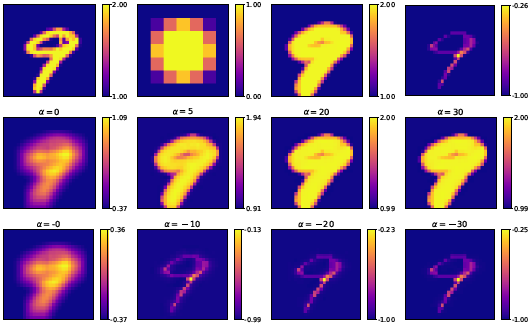
\includegraphics[scale=0.9]{images/SMorph}
    \label{fig:smorph}
\end{figure}
